\batchmode
\documentclass[twoside]{book}

% Packages required by doxygen
\usepackage{fixltx2e}
\usepackage{calc}
\usepackage{doxygen}
\usepackage[export]{adjustbox} % also loads graphicx
\usepackage{graphicx}
\usepackage[utf8]{inputenc}
\usepackage{makeidx}
\usepackage{multicol}
\usepackage{multirow}
\PassOptionsToPackage{warn}{textcomp}
\usepackage{textcomp}
\usepackage[nointegrals]{wasysym}
\usepackage[table]{xcolor}

% Font selection
\usepackage[T1]{fontenc}
\usepackage[scaled=.90]{helvet}
\usepackage{courier}
\usepackage{amssymb}
\usepackage{sectsty}
\renewcommand{\familydefault}{\sfdefault}
\allsectionsfont{%
  \fontseries{bc}\selectfont%
  \color{darkgray}%
}
\renewcommand{\DoxyLabelFont}{%
  \fontseries{bc}\selectfont%
  \color{darkgray}%
}
\newcommand{\+}{\discretionary{\mbox{\scriptsize$\hookleftarrow$}}{}{}}

% Page & text layout
\usepackage{geometry}
\geometry{%
  a4paper,%
  top=2.5cm,%
  bottom=2.5cm,%
  left=2.5cm,%
  right=2.5cm%
}
\tolerance=750
\hfuzz=15pt
\hbadness=750
\setlength{\emergencystretch}{15pt}
\setlength{\parindent}{0cm}
\setlength{\parskip}{3ex plus 2ex minus 2ex}
\makeatletter
\renewcommand{\paragraph}{%
  \@startsection{paragraph}{4}{0ex}{-1.0ex}{1.0ex}{%
    \normalfont\normalsize\bfseries\SS@parafont%
  }%
}
\renewcommand{\subparagraph}{%
  \@startsection{subparagraph}{5}{0ex}{-1.0ex}{1.0ex}{%
    \normalfont\normalsize\bfseries\SS@subparafont%
  }%
}
\makeatother

% Headers & footers
\usepackage{fancyhdr}
\pagestyle{fancyplain}
\fancyhead[LE]{\fancyplain{}{\bfseries\thepage}}
\fancyhead[CE]{\fancyplain{}{}}
\fancyhead[RE]{\fancyplain{}{\bfseries\leftmark}}
\fancyhead[LO]{\fancyplain{}{\bfseries\rightmark}}
\fancyhead[CO]{\fancyplain{}{}}
\fancyhead[RO]{\fancyplain{}{\bfseries\thepage}}
\fancyfoot[LE]{\fancyplain{}{}}
\fancyfoot[CE]{\fancyplain{}{}}
\fancyfoot[RE]{\fancyplain{}{\bfseries\scriptsize Generated by Doxygen }}
\fancyfoot[LO]{\fancyplain{}{\bfseries\scriptsize Generated by Doxygen }}
\fancyfoot[CO]{\fancyplain{}{}}
\fancyfoot[RO]{\fancyplain{}{}}
\renewcommand{\footrulewidth}{0.4pt}
\renewcommand{\chaptermark}[1]{%
  \markboth{#1}{}%
}
\renewcommand{\sectionmark}[1]{%
  \markright{\thesection\ #1}%
}

% Indices & bibliography
\usepackage{natbib}
\usepackage[titles]{tocloft}
\setcounter{tocdepth}{3}
\setcounter{secnumdepth}{5}
\makeindex

% Packages requested by user
\usepackage{amsmath}
\usepackage{bm}

% Hyperlinks (required, but should be loaded last)
\usepackage{ifpdf}
\ifpdf
  \usepackage[pdftex,pagebackref=true]{hyperref}
\else
  \usepackage[ps2pdf,pagebackref=true]{hyperref}
\fi
\hypersetup{%
  colorlinks=true,%
  linkcolor=blue,%
  citecolor=blue,%
  unicode%
}

% Custom commands
\newcommand{\clearemptydoublepage}{%
  \newpage{\pagestyle{empty}\cleardoublepage}%
}

\usepackage{caption}
\captionsetup{labelsep=space,justification=centering,font={bf},singlelinecheck=off,skip=4pt,position=top}

%===== C O N T E N T S =====

\begin{document}

% Titlepage & ToC
\hypersetup{pageanchor=false,
             bookmarksnumbered=true,
             pdfencoding=unicode
            }
\pagenumbering{alph}
\pagenumbering{arabic}
\hypersetup{pageanchor=true}

%--- Begin generated contents ---
\chapter{The axisymmetric equations of linear elasticity}
\label{index}\hypertarget{index}{}\hypertarget{index_q}{}\section{A few quick questions...}\label{index_q}
Since {\ttfamily oomph-\/lib} is developed as open-\/source software, any evidence that the code is being downloaded and used is very helpful for us as it helps to justify our continued work on this project.

We would therefore be extremely grateful if you could provide the information requested in the form below. Pressing the \char`\"{}submit\char`\"{} button will get you to the actual download page.

{\bfseries Note\+:} 
\begin{DoxyItemize}
\item All information will be treated as confidential. 
\item If you provide your email address and check the appropriate box we will add you to our mailing list to inform you of upgrades and bug fixes to the code. Rest assured that the mailing list is {\bfseries very low volume} -- we have better things to do than to bombard you with email. 
\item If you still feel reluctant to provide any of the information requested, feel free to enter some dummy input. The form will check that {\bfseries some} information has been entered but entering your name as \char`\"{}\+Joe Cool\char`\"{} is perfectly acceptable -- this is to discourage people from not providing the information simply because they are too lazy to type... 
\end{DoxyItemize}



 







 

 \hypertarget{index_pdf}{}\section{P\+D\+F file}\label{index_pdf}
A \href{../latex/refman.pdf}{\tt pdf version} of this document is available. \end{document}

\chapter{Namespace Index}
\section{Namespace List}
Here is a list of all namespaces with brief descriptions\+:\begin{DoxyCompactList}
\item\contentsline{section}{\hyperlink{namespaceGlobal__Physical__Variables}{Global\+\_\+\+Physical\+\_\+\+Variables} \\*Global variables that represent physical properties }{\pageref{namespaceGlobal__Physical__Variables}}{}
\item\contentsline{section}{\hyperlink{namespaceoomph}{oomph} }{\pageref{namespaceoomph}}{}
\item\contentsline{section}{\hyperlink{namespacePhysical__Variables}{Physical\+\_\+\+Variables} \\*Namespace for the solution of 2D linear shell equation }{\pageref{namespacePhysical__Variables}}{}
\end{DoxyCompactList}

\chapter{Hierarchical Index}
\section{Class Hierarchy}
This inheritance list is sorted roughly, but not completely, alphabetically\+:\begin{DoxyCompactList}
\item Problem\begin{DoxyCompactList}
\item \contentsline{section}{Unstructured\+Solid\+Problem$<$ E\+L\+E\+M\+E\+NT $>$}{\pageref{classUnstructuredSolidProblem}}{}
\end{DoxyCompactList}
\end{DoxyCompactList}

\chapter{Class Index}
\section{Class List}
Here are the classes, structs, unions and interfaces with brief descriptions\+:\begin{DoxyCompactList}
\item\contentsline{section}{\hyperlink{classPMLProblem}{P\+M\+L\+Problem$<$ E\+L\+E\+M\+E\+N\+T $>$} }{\pageref{classPMLProblem}}{}
\item\contentsline{section}{\hyperlink{classGlobalParameters_1_1TestPMLMapping}{Global\+Parameters\+::\+Test\+P\+M\+L\+Mapping} }{\pageref{classGlobalParameters_1_1TestPMLMapping}}{}
\end{DoxyCompactList}

\chapter{File Index}
\section{File List}
Here is a list of all files with brief descriptions\+:\begin{DoxyCompactList}
\item\contentsline{section}{\hyperlink{jeffery__orbit_8cc}{jeffery\+\_\+orbit.\+cc} }{\pageref{jeffery__orbit_8cc}}{}
\item\contentsline{section}{\hyperlink{jeffery__orbit_8txt__doxygenified_8h}{jeffery\+\_\+orbit.\+txt\+\_\+doxygenified.\+h} }{\pageref{jeffery__orbit_8txt__doxygenified_8h}}{}
\item\contentsline{section}{\hyperlink{my__taylor__hood__elements_8h}{my\+\_\+taylor\+\_\+hood\+\_\+elements.\+h} }{\pageref{my__taylor__hood__elements_8h}}{}
\end{DoxyCompactList}

\chapter{Namespace Documentation}
\hypertarget{namespaceGlobal__Parameters}{}\section{Global\+\_\+\+Parameters Namespace Reference}
\label{namespaceGlobal__Parameters}\index{Global\+\_\+\+Parameters@{Global\+\_\+\+Parameters}}


Global variables.  


\subsection*{Functions}
\begin{DoxyCompactItemize}
\item 
void \hyperlink{namespaceGlobal__Parameters_a200109847bf4cc26da4d00e8d68d569e}{gravity} (const double \&time, const Vector$<$ double $>$ \&xi, Vector$<$ double $>$ \&b)
\begin{DoxyCompactList}\small\item\em Non-\/dimensional gravity as body force. \end{DoxyCompactList}\item 
double \hyperlink{namespaceGlobal__Parameters_a536aa5314a6cdb36af852e9513351d55}{flux} (const double \&t)
\begin{DoxyCompactList}\small\item\em Flux increases between Min\+\_\+flux and Max\+\_\+flux over period Ramp\+\_\+period. \end{DoxyCompactList}\item 
void \hyperlink{namespaceGlobal__Parameters_a8c333f9041cad78d5c0160a8e2c169f5}{set\+\_\+parameters} (const string \&case\+\_\+id)
\begin{DoxyCompactList}\small\item\em Set parameters for the various test cases. \end{DoxyCompactList}\end{DoxyCompactItemize}
\subsection*{Variables}
\begin{DoxyCompactItemize}
\item 
string \hyperlink{namespaceGlobal__Parameters_a887474a9be53363806b4de417f660dba}{Case\+\_\+\+ID} =\char`\"{}F\+S\+I1\char`\"{}
\begin{DoxyCompactList}\small\item\em Default case ID. \end{DoxyCompactList}\item 
double \hyperlink{namespaceGlobal__Parameters_a9d72e94a9305c6a310940a6a427ebe06}{Re} =20.\+0
\begin{DoxyCompactList}\small\item\em Reynolds number (default assignment for F\+S\+I1 test case) \end{DoxyCompactList}\item 
double \hyperlink{namespaceGlobal__Parameters_af1af40a0df651e86bc1be273fafa98da}{St} =0.\+5
\begin{DoxyCompactList}\small\item\em Strouhal number (default assignment for F\+S\+I1 test case) \end{DoxyCompactList}\item 
double \hyperlink{namespaceGlobal__Parameters_a7a59a32365e87566069e458dc83bd18a}{Re\+St} =10.\+0
\begin{DoxyCompactList}\small\item\em Product of Reynolds and Strouhal numbers (default assignment for F\+S\+I1 test case) \end{DoxyCompactList}\item 
double \hyperlink{namespaceGlobal__Parameters_a7814fddf663e56168174a42d2cd6b4c1}{Q} =1.\+429e-\/6
\begin{DoxyCompactList}\small\item\em F\+SI parameter (default assignment for F\+S\+I1 test case) \end{DoxyCompactList}\item 
double \hyperlink{namespaceGlobal__Parameters_a517d4c31b8bce6563c2f605266dd9679}{Density\+\_\+ratio} =1.\+0
\begin{DoxyCompactList}\small\item\em Density ratio (solid to fluid; default assignment for F\+S\+I1 test case) \end{DoxyCompactList}\item 
double \hyperlink{namespaceGlobal__Parameters_ab360628e7830e43e355ce5768f6d6a6c}{H} =0.\+2
\begin{DoxyCompactList}\small\item\em Height of flag. \end{DoxyCompactList}\item 
double \hyperlink{namespaceGlobal__Parameters_a0f0247cc83ba202413b50e7b4b7fceb0}{Centre\+\_\+x} =2.\+0
\begin{DoxyCompactList}\small\item\em x position of centre of cylinder \end{DoxyCompactList}\item 
double \hyperlink{namespaceGlobal__Parameters_af41282d812fdff4867e3d8c825886290}{Centre\+\_\+y} =2.\+0
\begin{DoxyCompactList}\small\item\em y position of centre of cylinder \end{DoxyCompactList}\item 
double \hyperlink{namespaceGlobal__Parameters_a126c1e491ef187867b6b7bfb52b476ad}{Radius} =0.\+5
\begin{DoxyCompactList}\small\item\em Radius of cylinder. \end{DoxyCompactList}\item 
Constitutive\+Law $\ast$ \hyperlink{namespaceGlobal__Parameters_adbd1f040f375c96fe56b3f475f7dbec2}{Constitutive\+\_\+law\+\_\+pt} =0
\begin{DoxyCompactList}\small\item\em Pointer to constitutive law. \end{DoxyCompactList}\item 
double \hyperlink{namespaceGlobal__Parameters_a3e3428638f89f970fcf2148b0bab1465}{Lambda\+\_\+sq} =0.\+0
\begin{DoxyCompactList}\small\item\em Timescale ratio for solid (dependent parameter assigned in \hyperlink{namespaceGlobal__Parameters_a8c333f9041cad78d5c0160a8e2c169f5}{set\+\_\+parameters()}) \end{DoxyCompactList}\item 
double \hyperlink{namespaceGlobal__Parameters_ab29c9f716872de235c78e62bce2c4109}{Dt} =0.\+1
\begin{DoxyCompactList}\small\item\em Timestep. \end{DoxyCompactList}\item 
bool \hyperlink{namespaceGlobal__Parameters_aac13d615d2acd78d22a3137ffd62f7aa}{Ignore\+\_\+fluid\+\_\+loading} =false
\begin{DoxyCompactList}\small\item\em Ignore fluid (default assignment for F\+S\+I1 test case) \end{DoxyCompactList}\item 
double \hyperlink{namespaceGlobal__Parameters_aa3dfbdb1b2fd80d516850f66c96b6fd0}{E} =1.\+0
\begin{DoxyCompactList}\small\item\em Elastic modulus. \end{DoxyCompactList}\item 
double \hyperlink{namespaceGlobal__Parameters_a20fccdcfa2c15ad8b951b9ada3bb1661}{Nu} =0.\+4
\begin{DoxyCompactList}\small\item\em Poisson\textquotesingle{}s ratio. \end{DoxyCompactList}\item 
double \hyperlink{namespaceGlobal__Parameters_a335000b5db4206486a116ae0468d2d0c}{Gravity} =0.\+0
\begin{DoxyCompactList}\small\item\em Non-\/dim gravity (default assignment for F\+S\+I1 test case) \end{DoxyCompactList}\item 
double \hyperlink{namespaceGlobal__Parameters_af6afcca0b1ffdf88144f99cdfed18d3b}{Ramp\+\_\+period} =2.\+0
\begin{DoxyCompactList}\small\item\em Period for ramping up in flux. \end{DoxyCompactList}\item 
double \hyperlink{namespaceGlobal__Parameters_a5aabde2d31d07e5d0a84f6ff02c263dc}{Min\+\_\+flux} =0.\+0
\begin{DoxyCompactList}\small\item\em Min. flux. \end{DoxyCompactList}\item 
double \hyperlink{namespaceGlobal__Parameters_a13f0d5d16393d21bbc904aea5cff4ea4}{Max\+\_\+flux} =1.\+0
\begin{DoxyCompactList}\small\item\em Max. flux. \end{DoxyCompactList}\end{DoxyCompactItemize}


\subsection{Detailed Description}
Global variables. 

\subsection{Function Documentation}
\mbox{\Hypertarget{namespaceGlobal__Parameters_a536aa5314a6cdb36af852e9513351d55}\label{namespaceGlobal__Parameters_a536aa5314a6cdb36af852e9513351d55}} 
\index{Global\+\_\+\+Parameters@{Global\+\_\+\+Parameters}!flux@{flux}}
\index{flux@{flux}!Global\+\_\+\+Parameters@{Global\+\_\+\+Parameters}}
\subsubsection{\texorpdfstring{flux()}{flux()}}
{\footnotesize\ttfamily double Global\+\_\+\+Parameters\+::flux (\begin{DoxyParamCaption}\item[{const double \&}]{t }\end{DoxyParamCaption})}



Flux increases between Min\+\_\+flux and Max\+\_\+flux over period Ramp\+\_\+period. 



Definition at line 132 of file turek\+\_\+flag.\+cc.



References Max\+\_\+flux, and Min\+\_\+flux.



Referenced by Turek\+Problem$<$ F\+L\+U\+I\+D\+\_\+\+E\+L\+E\+M\+E\+N\+T, S\+O\+L\+I\+D\+\_\+\+E\+L\+E\+M\+E\+N\+T $>$\+::actions\+\_\+before\+\_\+implicit\+\_\+timestep(), Turek\+Problem$<$ F\+L\+U\+I\+D\+\_\+\+E\+L\+E\+M\+E\+N\+T, S\+O\+L\+I\+D\+\_\+\+E\+L\+E\+M\+E\+N\+T $>$\+::doc\+\_\+solution(), and Turek\+Problem$<$ F\+L\+U\+I\+D\+\_\+\+E\+L\+E\+M\+E\+N\+T, S\+O\+L\+I\+D\+\_\+\+E\+L\+E\+M\+E\+N\+T $>$\+::\+Turek\+Problem().

\mbox{\Hypertarget{namespaceGlobal__Parameters_a200109847bf4cc26da4d00e8d68d569e}\label{namespaceGlobal__Parameters_a200109847bf4cc26da4d00e8d68d569e}} 
\index{Global\+\_\+\+Parameters@{Global\+\_\+\+Parameters}!gravity@{gravity}}
\index{gravity@{gravity}!Global\+\_\+\+Parameters@{Global\+\_\+\+Parameters}}
\subsubsection{\texorpdfstring{gravity()}{gravity()}}
{\footnotesize\ttfamily void Global\+\_\+\+Parameters\+::gravity (\begin{DoxyParamCaption}\item[{const double \&}]{time,  }\item[{const Vector$<$ double $>$ \&}]{xi,  }\item[{Vector$<$ double $>$ \&}]{b }\end{DoxyParamCaption})}



Non-\/dimensional gravity as body force. 



Definition at line 113 of file turek\+\_\+flag.\+cc.



References Gravity.



Referenced by Turek\+Problem$<$ F\+L\+U\+I\+D\+\_\+\+E\+L\+E\+M\+E\+N\+T, S\+O\+L\+I\+D\+\_\+\+E\+L\+E\+M\+E\+N\+T $>$\+::\+Turek\+Problem().

\mbox{\Hypertarget{namespaceGlobal__Parameters_a8c333f9041cad78d5c0160a8e2c169f5}\label{namespaceGlobal__Parameters_a8c333f9041cad78d5c0160a8e2c169f5}} 
\index{Global\+\_\+\+Parameters@{Global\+\_\+\+Parameters}!set\+\_\+parameters@{set\+\_\+parameters}}
\index{set\+\_\+parameters@{set\+\_\+parameters}!Global\+\_\+\+Parameters@{Global\+\_\+\+Parameters}}
\subsubsection{\texorpdfstring{set\+\_\+parameters()}{set\_parameters()}}
{\footnotesize\ttfamily void Global\+\_\+\+Parameters\+::set\+\_\+parameters (\begin{DoxyParamCaption}\item[{const string \&}]{case\+\_\+id }\end{DoxyParamCaption})}



Set parameters for the various test cases. 



Definition at line 147 of file turek\+\_\+flag.\+cc.



References St.



Referenced by main().



\subsection{Variable Documentation}
\mbox{\Hypertarget{namespaceGlobal__Parameters_a887474a9be53363806b4de417f660dba}\label{namespaceGlobal__Parameters_a887474a9be53363806b4de417f660dba}} 
\index{Global\+\_\+\+Parameters@{Global\+\_\+\+Parameters}!Case\+\_\+\+ID@{Case\+\_\+\+ID}}
\index{Case\+\_\+\+ID@{Case\+\_\+\+ID}!Global\+\_\+\+Parameters@{Global\+\_\+\+Parameters}}
\subsubsection{\texorpdfstring{Case\+\_\+\+ID}{Case\_ID}}
{\footnotesize\ttfamily string Global\+\_\+\+Parameters\+::\+Case\+\_\+\+ID =\char`\"{}F\+S\+I1\char`\"{}}



Default case ID. 



Definition at line 59 of file turek\+\_\+flag.\+cc.



Referenced by main().

\mbox{\Hypertarget{namespaceGlobal__Parameters_a0f0247cc83ba202413b50e7b4b7fceb0}\label{namespaceGlobal__Parameters_a0f0247cc83ba202413b50e7b4b7fceb0}} 
\index{Global\+\_\+\+Parameters@{Global\+\_\+\+Parameters}!Centre\+\_\+x@{Centre\+\_\+x}}
\index{Centre\+\_\+x@{Centre\+\_\+x}!Global\+\_\+\+Parameters@{Global\+\_\+\+Parameters}}
\subsubsection{\texorpdfstring{Centre\+\_\+x}{Centre\_x}}
{\footnotesize\ttfamily double Global\+\_\+\+Parameters\+::\+Centre\+\_\+x =2.\+0}



x position of centre of cylinder 



Definition at line 82 of file turek\+\_\+flag.\+cc.



Referenced by Turek\+Problem$<$ F\+L\+U\+I\+D\+\_\+\+E\+L\+E\+M\+E\+N\+T, S\+O\+L\+I\+D\+\_\+\+E\+L\+E\+M\+E\+N\+T $>$\+::\+Turek\+Problem().

\mbox{\Hypertarget{namespaceGlobal__Parameters_af41282d812fdff4867e3d8c825886290}\label{namespaceGlobal__Parameters_af41282d812fdff4867e3d8c825886290}} 
\index{Global\+\_\+\+Parameters@{Global\+\_\+\+Parameters}!Centre\+\_\+y@{Centre\+\_\+y}}
\index{Centre\+\_\+y@{Centre\+\_\+y}!Global\+\_\+\+Parameters@{Global\+\_\+\+Parameters}}
\subsubsection{\texorpdfstring{Centre\+\_\+y}{Centre\_y}}
{\footnotesize\ttfamily double Global\+\_\+\+Parameters\+::\+Centre\+\_\+y =2.\+0}



y position of centre of cylinder 



Definition at line 85 of file turek\+\_\+flag.\+cc.



Referenced by Turek\+Problem$<$ F\+L\+U\+I\+D\+\_\+\+E\+L\+E\+M\+E\+N\+T, S\+O\+L\+I\+D\+\_\+\+E\+L\+E\+M\+E\+N\+T $>$\+::\+Turek\+Problem().

\mbox{\Hypertarget{namespaceGlobal__Parameters_adbd1f040f375c96fe56b3f475f7dbec2}\label{namespaceGlobal__Parameters_adbd1f040f375c96fe56b3f475f7dbec2}} 
\index{Global\+\_\+\+Parameters@{Global\+\_\+\+Parameters}!Constitutive\+\_\+law\+\_\+pt@{Constitutive\+\_\+law\+\_\+pt}}
\index{Constitutive\+\_\+law\+\_\+pt@{Constitutive\+\_\+law\+\_\+pt}!Global\+\_\+\+Parameters@{Global\+\_\+\+Parameters}}
\subsubsection{\texorpdfstring{Constitutive\+\_\+law\+\_\+pt}{Constitutive\_law\_pt}}
{\footnotesize\ttfamily Constitutive\+Law$\ast$ Global\+\_\+\+Parameters\+::\+Constitutive\+\_\+law\+\_\+pt =0}



Pointer to constitutive law. 



Definition at line 91 of file turek\+\_\+flag.\+cc.



Referenced by Turek\+Problem$<$ F\+L\+U\+I\+D\+\_\+\+E\+L\+E\+M\+E\+N\+T, S\+O\+L\+I\+D\+\_\+\+E\+L\+E\+M\+E\+N\+T $>$\+::\+Turek\+Problem().

\mbox{\Hypertarget{namespaceGlobal__Parameters_a517d4c31b8bce6563c2f605266dd9679}\label{namespaceGlobal__Parameters_a517d4c31b8bce6563c2f605266dd9679}} 
\index{Global\+\_\+\+Parameters@{Global\+\_\+\+Parameters}!Density\+\_\+ratio@{Density\+\_\+ratio}}
\index{Density\+\_\+ratio@{Density\+\_\+ratio}!Global\+\_\+\+Parameters@{Global\+\_\+\+Parameters}}
\subsubsection{\texorpdfstring{Density\+\_\+ratio}{Density\_ratio}}
{\footnotesize\ttfamily double Global\+\_\+\+Parameters\+::\+Density\+\_\+ratio =1.\+0}



Density ratio (solid to fluid; default assignment for F\+S\+I1 test case) 



Definition at line 76 of file turek\+\_\+flag.\+cc.

\mbox{\Hypertarget{namespaceGlobal__Parameters_ab29c9f716872de235c78e62bce2c4109}\label{namespaceGlobal__Parameters_ab29c9f716872de235c78e62bce2c4109}} 
\index{Global\+\_\+\+Parameters@{Global\+\_\+\+Parameters}!Dt@{Dt}}
\index{Dt@{Dt}!Global\+\_\+\+Parameters@{Global\+\_\+\+Parameters}}
\subsubsection{\texorpdfstring{Dt}{Dt}}
{\footnotesize\ttfamily double Global\+\_\+\+Parameters\+::\+Dt =0.\+1}



Timestep. 



Definition at line 98 of file turek\+\_\+flag.\+cc.



Referenced by main().

\mbox{\Hypertarget{namespaceGlobal__Parameters_aa3dfbdb1b2fd80d516850f66c96b6fd0}\label{namespaceGlobal__Parameters_aa3dfbdb1b2fd80d516850f66c96b6fd0}} 
\index{Global\+\_\+\+Parameters@{Global\+\_\+\+Parameters}!E@{E}}
\index{E@{E}!Global\+\_\+\+Parameters@{Global\+\_\+\+Parameters}}
\subsubsection{\texorpdfstring{E}{E}}
{\footnotesize\ttfamily double Global\+\_\+\+Parameters\+::E =1.\+0}



Elastic modulus. 



Definition at line 104 of file turek\+\_\+flag.\+cc.

\mbox{\Hypertarget{namespaceGlobal__Parameters_a335000b5db4206486a116ae0468d2d0c}\label{namespaceGlobal__Parameters_a335000b5db4206486a116ae0468d2d0c}} 
\index{Global\+\_\+\+Parameters@{Global\+\_\+\+Parameters}!Gravity@{Gravity}}
\index{Gravity@{Gravity}!Global\+\_\+\+Parameters@{Global\+\_\+\+Parameters}}
\subsubsection{\texorpdfstring{Gravity}{Gravity}}
{\footnotesize\ttfamily double Global\+\_\+\+Parameters\+::\+Gravity =0.\+0}



Non-\/dim gravity (default assignment for F\+S\+I1 test case) 



Definition at line 110 of file turek\+\_\+flag.\+cc.



Referenced by gravity().

\mbox{\Hypertarget{namespaceGlobal__Parameters_ab360628e7830e43e355ce5768f6d6a6c}\label{namespaceGlobal__Parameters_ab360628e7830e43e355ce5768f6d6a6c}} 
\index{Global\+\_\+\+Parameters@{Global\+\_\+\+Parameters}!H@{H}}
\index{H@{H}!Global\+\_\+\+Parameters@{Global\+\_\+\+Parameters}}
\subsubsection{\texorpdfstring{H}{H}}
{\footnotesize\ttfamily double Global\+\_\+\+Parameters\+::H =0.\+2}



Height of flag. 



Definition at line 79 of file turek\+\_\+flag.\+cc.



Referenced by Turek\+Problem$<$ F\+L\+U\+I\+D\+\_\+\+E\+L\+E\+M\+E\+N\+T, S\+O\+L\+I\+D\+\_\+\+E\+L\+E\+M\+E\+N\+T $>$\+::\+Turek\+Problem().

\mbox{\Hypertarget{namespaceGlobal__Parameters_aac13d615d2acd78d22a3137ffd62f7aa}\label{namespaceGlobal__Parameters_aac13d615d2acd78d22a3137ffd62f7aa}} 
\index{Global\+\_\+\+Parameters@{Global\+\_\+\+Parameters}!Ignore\+\_\+fluid\+\_\+loading@{Ignore\+\_\+fluid\+\_\+loading}}
\index{Ignore\+\_\+fluid\+\_\+loading@{Ignore\+\_\+fluid\+\_\+loading}!Global\+\_\+\+Parameters@{Global\+\_\+\+Parameters}}
\subsubsection{\texorpdfstring{Ignore\+\_\+fluid\+\_\+loading}{Ignore\_fluid\_loading}}
{\footnotesize\ttfamily bool Global\+\_\+\+Parameters\+::\+Ignore\+\_\+fluid\+\_\+loading =false}



Ignore fluid (default assignment for F\+S\+I1 test case) 



Definition at line 101 of file turek\+\_\+flag.\+cc.



Referenced by Turek\+Problem$<$ F\+L\+U\+I\+D\+\_\+\+E\+L\+E\+M\+E\+N\+T, S\+O\+L\+I\+D\+\_\+\+E\+L\+E\+M\+E\+N\+T $>$\+::actions\+\_\+after\+\_\+adapt(), and Turek\+Problem$<$ F\+L\+U\+I\+D\+\_\+\+E\+L\+E\+M\+E\+N\+T, S\+O\+L\+I\+D\+\_\+\+E\+L\+E\+M\+E\+N\+T $>$\+::\+Turek\+Problem().

\mbox{\Hypertarget{namespaceGlobal__Parameters_a3e3428638f89f970fcf2148b0bab1465}\label{namespaceGlobal__Parameters_a3e3428638f89f970fcf2148b0bab1465}} 
\index{Global\+\_\+\+Parameters@{Global\+\_\+\+Parameters}!Lambda\+\_\+sq@{Lambda\+\_\+sq}}
\index{Lambda\+\_\+sq@{Lambda\+\_\+sq}!Global\+\_\+\+Parameters@{Global\+\_\+\+Parameters}}
\subsubsection{\texorpdfstring{Lambda\+\_\+sq}{Lambda\_sq}}
{\footnotesize\ttfamily double Global\+\_\+\+Parameters\+::\+Lambda\+\_\+sq =0.\+0}



Timescale ratio for solid (dependent parameter assigned in \hyperlink{namespaceGlobal__Parameters_a8c333f9041cad78d5c0160a8e2c169f5}{set\+\_\+parameters()}) 



Definition at line 95 of file turek\+\_\+flag.\+cc.



Referenced by Turek\+Problem$<$ F\+L\+U\+I\+D\+\_\+\+E\+L\+E\+M\+E\+N\+T, S\+O\+L\+I\+D\+\_\+\+E\+L\+E\+M\+E\+N\+T $>$\+::\+Turek\+Problem().

\mbox{\Hypertarget{namespaceGlobal__Parameters_a13f0d5d16393d21bbc904aea5cff4ea4}\label{namespaceGlobal__Parameters_a13f0d5d16393d21bbc904aea5cff4ea4}} 
\index{Global\+\_\+\+Parameters@{Global\+\_\+\+Parameters}!Max\+\_\+flux@{Max\+\_\+flux}}
\index{Max\+\_\+flux@{Max\+\_\+flux}!Global\+\_\+\+Parameters@{Global\+\_\+\+Parameters}}
\subsubsection{\texorpdfstring{Max\+\_\+flux}{Max\_flux}}
{\footnotesize\ttfamily double Global\+\_\+\+Parameters\+::\+Max\+\_\+flux =1.\+0}



Max. flux. 



Definition at line 128 of file turek\+\_\+flag.\+cc.



Referenced by flux().

\mbox{\Hypertarget{namespaceGlobal__Parameters_a5aabde2d31d07e5d0a84f6ff02c263dc}\label{namespaceGlobal__Parameters_a5aabde2d31d07e5d0a84f6ff02c263dc}} 
\index{Global\+\_\+\+Parameters@{Global\+\_\+\+Parameters}!Min\+\_\+flux@{Min\+\_\+flux}}
\index{Min\+\_\+flux@{Min\+\_\+flux}!Global\+\_\+\+Parameters@{Global\+\_\+\+Parameters}}
\subsubsection{\texorpdfstring{Min\+\_\+flux}{Min\_flux}}
{\footnotesize\ttfamily double Global\+\_\+\+Parameters\+::\+Min\+\_\+flux =0.\+0}



Min. flux. 



Definition at line 125 of file turek\+\_\+flag.\+cc.



Referenced by flux().

\mbox{\Hypertarget{namespaceGlobal__Parameters_a20fccdcfa2c15ad8b951b9ada3bb1661}\label{namespaceGlobal__Parameters_a20fccdcfa2c15ad8b951b9ada3bb1661}} 
\index{Global\+\_\+\+Parameters@{Global\+\_\+\+Parameters}!Nu@{Nu}}
\index{Nu@{Nu}!Global\+\_\+\+Parameters@{Global\+\_\+\+Parameters}}
\subsubsection{\texorpdfstring{Nu}{Nu}}
{\footnotesize\ttfamily double Global\+\_\+\+Parameters\+::\+Nu =0.\+4}



Poisson\textquotesingle{}s ratio. 



Definition at line 107 of file turek\+\_\+flag.\+cc.

\mbox{\Hypertarget{namespaceGlobal__Parameters_a7814fddf663e56168174a42d2cd6b4c1}\label{namespaceGlobal__Parameters_a7814fddf663e56168174a42d2cd6b4c1}} 
\index{Global\+\_\+\+Parameters@{Global\+\_\+\+Parameters}!Q@{Q}}
\index{Q@{Q}!Global\+\_\+\+Parameters@{Global\+\_\+\+Parameters}}
\subsubsection{\texorpdfstring{Q}{Q}}
{\footnotesize\ttfamily double Global\+\_\+\+Parameters\+::Q =1.\+429e-\/6}



F\+SI parameter (default assignment for F\+S\+I1 test case) 



Definition at line 72 of file turek\+\_\+flag.\+cc.



Referenced by Turek\+Problem$<$ F\+L\+U\+I\+D\+\_\+\+E\+L\+E\+M\+E\+N\+T, S\+O\+L\+I\+D\+\_\+\+E\+L\+E\+M\+E\+N\+T $>$\+::\+Turek\+Problem().

\mbox{\Hypertarget{namespaceGlobal__Parameters_a126c1e491ef187867b6b7bfb52b476ad}\label{namespaceGlobal__Parameters_a126c1e491ef187867b6b7bfb52b476ad}} 
\index{Global\+\_\+\+Parameters@{Global\+\_\+\+Parameters}!Radius@{Radius}}
\index{Radius@{Radius}!Global\+\_\+\+Parameters@{Global\+\_\+\+Parameters}}
\subsubsection{\texorpdfstring{Radius}{Radius}}
{\footnotesize\ttfamily double Global\+\_\+\+Parameters\+::\+Radius =0.\+5}



Radius of cylinder. 



Definition at line 88 of file turek\+\_\+flag.\+cc.



Referenced by Turek\+Problem$<$ F\+L\+U\+I\+D\+\_\+\+E\+L\+E\+M\+E\+N\+T, S\+O\+L\+I\+D\+\_\+\+E\+L\+E\+M\+E\+N\+T $>$\+::\+Turek\+Problem().

\mbox{\Hypertarget{namespaceGlobal__Parameters_af6afcca0b1ffdf88144f99cdfed18d3b}\label{namespaceGlobal__Parameters_af6afcca0b1ffdf88144f99cdfed18d3b}} 
\index{Global\+\_\+\+Parameters@{Global\+\_\+\+Parameters}!Ramp\+\_\+period@{Ramp\+\_\+period}}
\index{Ramp\+\_\+period@{Ramp\+\_\+period}!Global\+\_\+\+Parameters@{Global\+\_\+\+Parameters}}
\subsubsection{\texorpdfstring{Ramp\+\_\+period}{Ramp\_period}}
{\footnotesize\ttfamily double Global\+\_\+\+Parameters\+::\+Ramp\+\_\+period =2.\+0}



Period for ramping up in flux. 



Definition at line 122 of file turek\+\_\+flag.\+cc.

\mbox{\Hypertarget{namespaceGlobal__Parameters_a9d72e94a9305c6a310940a6a427ebe06}\label{namespaceGlobal__Parameters_a9d72e94a9305c6a310940a6a427ebe06}} 
\index{Global\+\_\+\+Parameters@{Global\+\_\+\+Parameters}!Re@{Re}}
\index{Re@{Re}!Global\+\_\+\+Parameters@{Global\+\_\+\+Parameters}}
\subsubsection{\texorpdfstring{Re}{Re}}
{\footnotesize\ttfamily double Global\+\_\+\+Parameters\+::\+Re =20.\+0}



Reynolds number (default assignment for F\+S\+I1 test case) 



Definition at line 62 of file turek\+\_\+flag.\+cc.



Referenced by Turek\+Problem$<$ F\+L\+U\+I\+D\+\_\+\+E\+L\+E\+M\+E\+N\+T, S\+O\+L\+I\+D\+\_\+\+E\+L\+E\+M\+E\+N\+T $>$\+::\+Turek\+Problem().

\mbox{\Hypertarget{namespaceGlobal__Parameters_a7a59a32365e87566069e458dc83bd18a}\label{namespaceGlobal__Parameters_a7a59a32365e87566069e458dc83bd18a}} 
\index{Global\+\_\+\+Parameters@{Global\+\_\+\+Parameters}!Re\+St@{Re\+St}}
\index{Re\+St@{Re\+St}!Global\+\_\+\+Parameters@{Global\+\_\+\+Parameters}}
\subsubsection{\texorpdfstring{Re\+St}{ReSt}}
{\footnotesize\ttfamily double Global\+\_\+\+Parameters\+::\+Re\+St =10.\+0}



Product of Reynolds and Strouhal numbers (default assignment for F\+S\+I1 test case) 



Definition at line 69 of file turek\+\_\+flag.\+cc.



Referenced by Turek\+Problem$<$ F\+L\+U\+I\+D\+\_\+\+E\+L\+E\+M\+E\+N\+T, S\+O\+L\+I\+D\+\_\+\+E\+L\+E\+M\+E\+N\+T $>$\+::\+Turek\+Problem().

\mbox{\Hypertarget{namespaceGlobal__Parameters_af1af40a0df651e86bc1be273fafa98da}\label{namespaceGlobal__Parameters_af1af40a0df651e86bc1be273fafa98da}} 
\index{Global\+\_\+\+Parameters@{Global\+\_\+\+Parameters}!St@{St}}
\index{St@{St}!Global\+\_\+\+Parameters@{Global\+\_\+\+Parameters}}
\subsubsection{\texorpdfstring{St}{St}}
{\footnotesize\ttfamily double Global\+\_\+\+Parameters\+::\+St =0.\+5}



Strouhal number (default assignment for F\+S\+I1 test case) 



Definition at line 65 of file turek\+\_\+flag.\+cc.



Referenced by set\+\_\+parameters(), and Turek\+Problem$<$ F\+L\+U\+I\+D\+\_\+\+E\+L\+E\+M\+E\+N\+T, S\+O\+L\+I\+D\+\_\+\+E\+L\+E\+M\+E\+N\+T $>$\+::\+Turek\+Problem().


\chapter{Class Documentation}
\hypertarget{classAxisymmetricLinearElasticityProblem}{}\section{Axisymmetric\+Linear\+Elasticity\+Problem$<$ E\+L\+E\+M\+E\+NT, T\+I\+M\+E\+S\+T\+E\+P\+P\+ER $>$ Class Template Reference}
\label{classAxisymmetricLinearElasticityProblem}\index{Axisymmetric\+Linear\+Elasticity\+Problem$<$ E\+L\+E\+M\+E\+N\+T, T\+I\+M\+E\+S\+T\+E\+P\+P\+E\+R $>$@{Axisymmetric\+Linear\+Elasticity\+Problem$<$ E\+L\+E\+M\+E\+N\+T, T\+I\+M\+E\+S\+T\+E\+P\+P\+E\+R $>$}}
Inheritance diagram for Axisymmetric\+Linear\+Elasticity\+Problem$<$ E\+L\+E\+M\+E\+NT, T\+I\+M\+E\+S\+T\+E\+P\+P\+ER $>$\+:\begin{figure}[H]
\begin{center}
\leavevmode
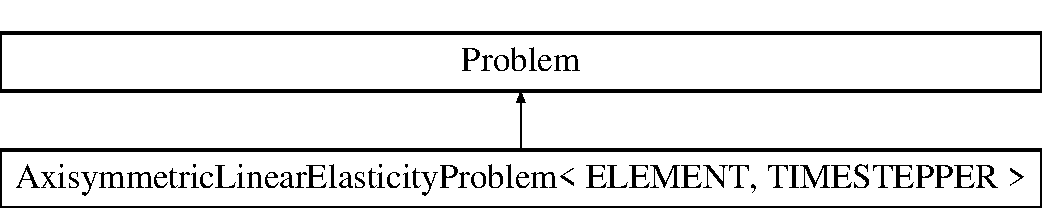
\includegraphics[height=2.000000cm]{classAxisymmetricLinearElasticityProblem}
\end{center}
\end{figure}
\subsection*{Public Member Functions}
\begin{DoxyCompactItemize}
\item 
\hyperlink{classAxisymmetricLinearElasticityProblem_aaa4da18227b8b20dfba1f67bad4907ed}{Axisymmetric\+Linear\+Elasticity\+Problem} ()
\begin{DoxyCompactList}\small\item\em Constructor\+: Pass number of elements in r and z directions, boundary locations and whether we are doing an impulsive start or not. \end{DoxyCompactList}\item 
void \hyperlink{classAxisymmetricLinearElasticityProblem_a25da062bc76af5ef30619a3f3ff3718f}{actions\+\_\+before\+\_\+newton\+\_\+solve} ()
\begin{DoxyCompactList}\small\item\em Update before solve is empty. \end{DoxyCompactList}\item 
void \hyperlink{classAxisymmetricLinearElasticityProblem_af9b01e082da514668a89df9213afbbd5}{actions\+\_\+after\+\_\+newton\+\_\+solve} ()
\begin{DoxyCompactList}\small\item\em Update after solve is empty. \end{DoxyCompactList}\item 
void \hyperlink{classAxisymmetricLinearElasticityProblem_a6ea18ecd60fd5878522ae6024cb57dee}{actions\+\_\+before\+\_\+implicit\+\_\+timestep} ()
\begin{DoxyCompactList}\small\item\em Actions before implicit timestep. \end{DoxyCompactList}\item 
void \hyperlink{classAxisymmetricLinearElasticityProblem_a6b0263b6f783652a1d8151948f4b9430}{set\+\_\+initial\+\_\+conditions} ()
\begin{DoxyCompactList}\small\item\em Set the initial conditions, either for an impulsive start or with history values for the time stepper. \end{DoxyCompactList}\item 
void \hyperlink{classAxisymmetricLinearElasticityProblem_ad6419d0572a6e869a5b9ba3c5aac3144}{set\+\_\+boundary\+\_\+conditions} ()
\begin{DoxyCompactList}\small\item\em Set the boundary conditions. \end{DoxyCompactList}\item 
void \hyperlink{classAxisymmetricLinearElasticityProblem_a370b76b9e2902242de018339d3aedd04}{doc\+\_\+solution} (Doc\+Info \&doc\+\_\+info)
\begin{DoxyCompactList}\small\item\em Doc the solution. \end{DoxyCompactList}\end{DoxyCompactItemize}
\subsection*{Private Member Functions}
\begin{DoxyCompactItemize}
\item 
void \hyperlink{classAxisymmetricLinearElasticityProblem_ab0cfde2632d6711b75744bcc2644ae04}{assign\+\_\+traction\+\_\+elements} ()
\begin{DoxyCompactList}\small\item\em Allocate traction elements on the bottom surface. \end{DoxyCompactList}\end{DoxyCompactItemize}
\subsection*{Private Attributes}
\begin{DoxyCompactItemize}
\item 
Mesh $\ast$ \hyperlink{classAxisymmetricLinearElasticityProblem_a49f2e786217cf28ebed1d828a4b06147}{Bulk\+\_\+mesh\+\_\+pt}
\begin{DoxyCompactList}\small\item\em Pointer to the bulk mesh. \end{DoxyCompactList}\item 
Mesh $\ast$ \hyperlink{classAxisymmetricLinearElasticityProblem_a62a8248651ee5b17b5168fe9158039dc}{Surface\+\_\+mesh\+\_\+pt}
\begin{DoxyCompactList}\small\item\em Pointer to the mesh of traction elements. \end{DoxyCompactList}\end{DoxyCompactItemize}


\subsection{Detailed Description}
\subsubsection*{template$<$class E\+L\+E\+M\+E\+NT, class T\+I\+M\+E\+S\+T\+E\+P\+P\+ER$>$\newline
class Axisymmetric\+Linear\+Elasticity\+Problem$<$ E\+L\+E\+M\+E\+N\+T, T\+I\+M\+E\+S\+T\+E\+P\+P\+E\+R $>$}

Class to validate time harmonic linear elasticity (Fourier decomposed) 

Definition at line 231 of file cylinder.\+cc.



\subsection{Constructor \& Destructor Documentation}
\mbox{\Hypertarget{classAxisymmetricLinearElasticityProblem_aaa4da18227b8b20dfba1f67bad4907ed}\label{classAxisymmetricLinearElasticityProblem_aaa4da18227b8b20dfba1f67bad4907ed}} 
\index{Axisymmetric\+Linear\+Elasticity\+Problem@{Axisymmetric\+Linear\+Elasticity\+Problem}!Axisymmetric\+Linear\+Elasticity\+Problem@{Axisymmetric\+Linear\+Elasticity\+Problem}}
\index{Axisymmetric\+Linear\+Elasticity\+Problem@{Axisymmetric\+Linear\+Elasticity\+Problem}!Axisymmetric\+Linear\+Elasticity\+Problem@{Axisymmetric\+Linear\+Elasticity\+Problem}}
\subsubsection{\texorpdfstring{Axisymmetric\+Linear\+Elasticity\+Problem()}{AxisymmetricLinearElasticityProblem()}}
{\footnotesize\ttfamily template$<$class E\+L\+E\+M\+E\+NT , class T\+I\+M\+E\+S\+T\+E\+P\+P\+ER $>$ \\
\hyperlink{classAxisymmetricLinearElasticityProblem}{Axisymmetric\+Linear\+Elasticity\+Problem}$<$ E\+L\+E\+M\+E\+NT, T\+I\+M\+E\+S\+T\+E\+P\+P\+ER $>$\+::\hyperlink{classAxisymmetricLinearElasticityProblem}{Axisymmetric\+Linear\+Elasticity\+Problem} (\begin{DoxyParamCaption}{ }\end{DoxyParamCaption})}



Constructor\+: Pass number of elements in r and z directions, boundary locations and whether we are doing an impulsive start or not. 

Problem constructor\+: Pass number of elements in coordinate directions and size of domain. 

Definition at line 281 of file cylinder.\+cc.



References Axisymmetric\+Linear\+Elasticity\+Problem$<$ E\+L\+E\+M\+E\+N\+T, T\+I\+M\+E\+S\+T\+E\+P\+P\+E\+R $>$\+::assign\+\_\+traction\+\_\+elements(), Global\+\_\+\+Parameters\+::body\+\_\+force(), Global\+\_\+\+Parameters\+::boundary\+\_\+traction(), Global\+\_\+\+Parameters\+::E, Global\+\_\+\+Parameters\+::\+Nr, Global\+\_\+\+Parameters\+::\+Nu, Global\+\_\+\+Parameters\+::\+Nz, Global\+\_\+\+Parameters\+::\+Omega\+\_\+sq, Global\+\_\+\+Parameters\+::\+Rmax, Global\+\_\+\+Parameters\+::\+Rmin, Global\+\_\+\+Parameters\+::\+Zmax, and Global\+\_\+\+Parameters\+::\+Zmin.



\subsection{Member Function Documentation}
\mbox{\Hypertarget{classAxisymmetricLinearElasticityProblem_af9b01e082da514668a89df9213afbbd5}\label{classAxisymmetricLinearElasticityProblem_af9b01e082da514668a89df9213afbbd5}} 
\index{Axisymmetric\+Linear\+Elasticity\+Problem@{Axisymmetric\+Linear\+Elasticity\+Problem}!actions\+\_\+after\+\_\+newton\+\_\+solve@{actions\+\_\+after\+\_\+newton\+\_\+solve}}
\index{actions\+\_\+after\+\_\+newton\+\_\+solve@{actions\+\_\+after\+\_\+newton\+\_\+solve}!Axisymmetric\+Linear\+Elasticity\+Problem@{Axisymmetric\+Linear\+Elasticity\+Problem}}
\subsubsection{\texorpdfstring{actions\+\_\+after\+\_\+newton\+\_\+solve()}{actions\_after\_newton\_solve()}}
{\footnotesize\ttfamily template$<$class E\+L\+E\+M\+E\+NT , class T\+I\+M\+E\+S\+T\+E\+P\+P\+ER $>$ \\
void \hyperlink{classAxisymmetricLinearElasticityProblem}{Axisymmetric\+Linear\+Elasticity\+Problem}$<$ E\+L\+E\+M\+E\+NT, T\+I\+M\+E\+S\+T\+E\+P\+P\+ER $>$\+::actions\+\_\+after\+\_\+newton\+\_\+solve (\begin{DoxyParamCaption}{ }\end{DoxyParamCaption})\hspace{0.3cm}{\ttfamily [inline]}}



Update after solve is empty. 



Definition at line 243 of file cylinder.\+cc.

\mbox{\Hypertarget{classAxisymmetricLinearElasticityProblem_a6ea18ecd60fd5878522ae6024cb57dee}\label{classAxisymmetricLinearElasticityProblem_a6ea18ecd60fd5878522ae6024cb57dee}} 
\index{Axisymmetric\+Linear\+Elasticity\+Problem@{Axisymmetric\+Linear\+Elasticity\+Problem}!actions\+\_\+before\+\_\+implicit\+\_\+timestep@{actions\+\_\+before\+\_\+implicit\+\_\+timestep}}
\index{actions\+\_\+before\+\_\+implicit\+\_\+timestep@{actions\+\_\+before\+\_\+implicit\+\_\+timestep}!Axisymmetric\+Linear\+Elasticity\+Problem@{Axisymmetric\+Linear\+Elasticity\+Problem}}
\subsubsection{\texorpdfstring{actions\+\_\+before\+\_\+implicit\+\_\+timestep()}{actions\_before\_implicit\_timestep()}}
{\footnotesize\ttfamily template$<$class E\+L\+E\+M\+E\+NT , class T\+I\+M\+E\+S\+T\+E\+P\+P\+ER $>$ \\
void \hyperlink{classAxisymmetricLinearElasticityProblem}{Axisymmetric\+Linear\+Elasticity\+Problem}$<$ E\+L\+E\+M\+E\+NT, T\+I\+M\+E\+S\+T\+E\+P\+P\+ER $>$\+::actions\+\_\+before\+\_\+implicit\+\_\+timestep (\begin{DoxyParamCaption}{ }\end{DoxyParamCaption})\hspace{0.3cm}{\ttfamily [inline]}}



Actions before implicit timestep. 



Definition at line 246 of file cylinder.\+cc.

\mbox{\Hypertarget{classAxisymmetricLinearElasticityProblem_a25da062bc76af5ef30619a3f3ff3718f}\label{classAxisymmetricLinearElasticityProblem_a25da062bc76af5ef30619a3f3ff3718f}} 
\index{Axisymmetric\+Linear\+Elasticity\+Problem@{Axisymmetric\+Linear\+Elasticity\+Problem}!actions\+\_\+before\+\_\+newton\+\_\+solve@{actions\+\_\+before\+\_\+newton\+\_\+solve}}
\index{actions\+\_\+before\+\_\+newton\+\_\+solve@{actions\+\_\+before\+\_\+newton\+\_\+solve}!Axisymmetric\+Linear\+Elasticity\+Problem@{Axisymmetric\+Linear\+Elasticity\+Problem}}
\subsubsection{\texorpdfstring{actions\+\_\+before\+\_\+newton\+\_\+solve()}{actions\_before\_newton\_solve()}}
{\footnotesize\ttfamily template$<$class E\+L\+E\+M\+E\+NT , class T\+I\+M\+E\+S\+T\+E\+P\+P\+ER $>$ \\
void \hyperlink{classAxisymmetricLinearElasticityProblem}{Axisymmetric\+Linear\+Elasticity\+Problem}$<$ E\+L\+E\+M\+E\+NT, T\+I\+M\+E\+S\+T\+E\+P\+P\+ER $>$\+::actions\+\_\+before\+\_\+newton\+\_\+solve (\begin{DoxyParamCaption}{ }\end{DoxyParamCaption})\hspace{0.3cm}{\ttfamily [inline]}}



Update before solve is empty. 



Definition at line 240 of file cylinder.\+cc.

\mbox{\Hypertarget{classAxisymmetricLinearElasticityProblem_ab0cfde2632d6711b75744bcc2644ae04}\label{classAxisymmetricLinearElasticityProblem_ab0cfde2632d6711b75744bcc2644ae04}} 
\index{Axisymmetric\+Linear\+Elasticity\+Problem@{Axisymmetric\+Linear\+Elasticity\+Problem}!assign\+\_\+traction\+\_\+elements@{assign\+\_\+traction\+\_\+elements}}
\index{assign\+\_\+traction\+\_\+elements@{assign\+\_\+traction\+\_\+elements}!Axisymmetric\+Linear\+Elasticity\+Problem@{Axisymmetric\+Linear\+Elasticity\+Problem}}
\subsubsection{\texorpdfstring{assign\+\_\+traction\+\_\+elements()}{assign\_traction\_elements()}}
{\footnotesize\ttfamily template$<$class E\+L\+E\+M\+E\+NT , class T\+I\+M\+E\+S\+T\+E\+P\+P\+ER $>$ \\
void \hyperlink{classAxisymmetricLinearElasticityProblem}{Axisymmetric\+Linear\+Elasticity\+Problem}$<$ E\+L\+E\+M\+E\+NT, T\+I\+M\+E\+S\+T\+E\+P\+P\+ER $>$\+::assign\+\_\+traction\+\_\+elements (\begin{DoxyParamCaption}{ }\end{DoxyParamCaption})\hspace{0.3cm}{\ttfamily [private]}}



Allocate traction elements on the bottom surface. 

Make traction elements along the boundary r=Rmin. 

Definition at line 392 of file cylinder.\+cc.



References Axisymmetric\+Linear\+Elasticity\+Problem$<$ E\+L\+E\+M\+E\+N\+T, T\+I\+M\+E\+S\+T\+E\+P\+P\+E\+R $>$\+::set\+\_\+initial\+\_\+conditions().



Referenced by Axisymmetric\+Linear\+Elasticity\+Problem$<$ E\+L\+E\+M\+E\+N\+T, T\+I\+M\+E\+S\+T\+E\+P\+P\+E\+R $>$\+::\+Axisymmetric\+Linear\+Elasticity\+Problem().

\mbox{\Hypertarget{classAxisymmetricLinearElasticityProblem_a370b76b9e2902242de018339d3aedd04}\label{classAxisymmetricLinearElasticityProblem_a370b76b9e2902242de018339d3aedd04}} 
\index{Axisymmetric\+Linear\+Elasticity\+Problem@{Axisymmetric\+Linear\+Elasticity\+Problem}!doc\+\_\+solution@{doc\+\_\+solution}}
\index{doc\+\_\+solution@{doc\+\_\+solution}!Axisymmetric\+Linear\+Elasticity\+Problem@{Axisymmetric\+Linear\+Elasticity\+Problem}}
\subsubsection{\texorpdfstring{doc\+\_\+solution()}{doc\_solution()}}
{\footnotesize\ttfamily template$<$class E\+L\+E\+M\+E\+NT , class T\+I\+M\+E\+S\+T\+E\+P\+P\+ER $>$ \\
void \hyperlink{classAxisymmetricLinearElasticityProblem}{Axisymmetric\+Linear\+Elasticity\+Problem}$<$ E\+L\+E\+M\+E\+NT, T\+I\+M\+E\+S\+T\+E\+P\+P\+ER $>$\+::doc\+\_\+solution (\begin{DoxyParamCaption}\item[{Doc\+Info \&}]{doc\+\_\+info }\end{DoxyParamCaption})}



Doc the solution. 



Definition at line 668 of file cylinder.\+cc.



References Global\+\_\+\+Parameters\+::exact\+\_\+solution().



Referenced by Axisymmetric\+Linear\+Elasticity\+Problem$<$ E\+L\+E\+M\+E\+N\+T, T\+I\+M\+E\+S\+T\+E\+P\+P\+E\+R $>$\+::set\+\_\+boundary\+\_\+conditions().

\mbox{\Hypertarget{classAxisymmetricLinearElasticityProblem_ad6419d0572a6e869a5b9ba3c5aac3144}\label{classAxisymmetricLinearElasticityProblem_ad6419d0572a6e869a5b9ba3c5aac3144}} 
\index{Axisymmetric\+Linear\+Elasticity\+Problem@{Axisymmetric\+Linear\+Elasticity\+Problem}!set\+\_\+boundary\+\_\+conditions@{set\+\_\+boundary\+\_\+conditions}}
\index{set\+\_\+boundary\+\_\+conditions@{set\+\_\+boundary\+\_\+conditions}!Axisymmetric\+Linear\+Elasticity\+Problem@{Axisymmetric\+Linear\+Elasticity\+Problem}}
\subsubsection{\texorpdfstring{set\+\_\+boundary\+\_\+conditions()}{set\_boundary\_conditions()}}
{\footnotesize\ttfamily template$<$class E\+L\+E\+M\+E\+NT , class T\+I\+M\+E\+S\+T\+E\+P\+P\+ER $>$ \\
void \hyperlink{classAxisymmetricLinearElasticityProblem}{Axisymmetric\+Linear\+Elasticity\+Problem}$<$ E\+L\+E\+M\+E\+NT, T\+I\+M\+E\+S\+T\+E\+P\+P\+ER $>$\+::set\+\_\+boundary\+\_\+conditions (\begin{DoxyParamCaption}{ }\end{DoxyParamCaption})}



Set the boundary conditions. 



Definition at line 578 of file cylinder.\+cc.



References Global\+\_\+\+Parameters\+::d2\+\_\+u\+\_\+r\+\_\+dt2(), Global\+\_\+\+Parameters\+::d2\+\_\+u\+\_\+theta\+\_\+dt2(), Global\+\_\+\+Parameters\+::d2\+\_\+u\+\_\+z\+\_\+dt2(), Global\+\_\+\+Parameters\+::d\+\_\+u\+\_\+r\+\_\+dt(), Global\+\_\+\+Parameters\+::d\+\_\+u\+\_\+theta\+\_\+dt(), Global\+\_\+\+Parameters\+::d\+\_\+u\+\_\+z\+\_\+dt(), Axisymmetric\+Linear\+Elasticity\+Problem$<$ E\+L\+E\+M\+E\+N\+T, T\+I\+M\+E\+S\+T\+E\+P\+P\+E\+R $>$\+::doc\+\_\+solution(), Global\+\_\+\+Parameters\+::exact\+\_\+solution(), Global\+\_\+\+Parameters\+::u\+\_\+r(), Global\+\_\+\+Parameters\+::u\+\_\+theta(), and Global\+\_\+\+Parameters\+::u\+\_\+z().



Referenced by Axisymmetric\+Linear\+Elasticity\+Problem$<$ E\+L\+E\+M\+E\+N\+T, T\+I\+M\+E\+S\+T\+E\+P\+P\+E\+R $>$\+::set\+\_\+initial\+\_\+conditions().

\mbox{\Hypertarget{classAxisymmetricLinearElasticityProblem_a6b0263b6f783652a1d8151948f4b9430}\label{classAxisymmetricLinearElasticityProblem_a6b0263b6f783652a1d8151948f4b9430}} 
\index{Axisymmetric\+Linear\+Elasticity\+Problem@{Axisymmetric\+Linear\+Elasticity\+Problem}!set\+\_\+initial\+\_\+conditions@{set\+\_\+initial\+\_\+conditions}}
\index{set\+\_\+initial\+\_\+conditions@{set\+\_\+initial\+\_\+conditions}!Axisymmetric\+Linear\+Elasticity\+Problem@{Axisymmetric\+Linear\+Elasticity\+Problem}}
\subsubsection{\texorpdfstring{set\+\_\+initial\+\_\+conditions()}{set\_initial\_conditions()}}
{\footnotesize\ttfamily template$<$class E\+L\+E\+M\+E\+NT , class T\+I\+M\+E\+S\+T\+E\+P\+P\+ER $>$ \\
void \hyperlink{classAxisymmetricLinearElasticityProblem}{Axisymmetric\+Linear\+Elasticity\+Problem}$<$ E\+L\+E\+M\+E\+NT, T\+I\+M\+E\+S\+T\+E\+P\+P\+ER $>$\+::set\+\_\+initial\+\_\+conditions (\begin{DoxyParamCaption}{ }\end{DoxyParamCaption})}



Set the initial conditions, either for an impulsive start or with history values for the time stepper. 

Set the initial conditions (history values) 

Definition at line 420 of file cylinder.\+cc.



References Global\+\_\+\+Parameters\+::d2\+\_\+u\+\_\+r\+\_\+dt2(), Global\+\_\+\+Parameters\+::d2\+\_\+u\+\_\+theta\+\_\+dt2(), Global\+\_\+\+Parameters\+::d2\+\_\+u\+\_\+z\+\_\+dt2(), Global\+\_\+\+Parameters\+::d\+\_\+u\+\_\+r\+\_\+dt(), Global\+\_\+\+Parameters\+::d\+\_\+u\+\_\+theta\+\_\+dt(), Global\+\_\+\+Parameters\+::d\+\_\+u\+\_\+z\+\_\+dt(), Axisymmetric\+Linear\+Elasticity\+Problem$<$ E\+L\+E\+M\+E\+N\+T, T\+I\+M\+E\+S\+T\+E\+P\+P\+E\+R $>$\+::set\+\_\+boundary\+\_\+conditions(), Global\+\_\+\+Parameters\+::u\+\_\+r(), Global\+\_\+\+Parameters\+::u\+\_\+theta(), and Global\+\_\+\+Parameters\+::u\+\_\+z().



Referenced by Axisymmetric\+Linear\+Elasticity\+Problem$<$ E\+L\+E\+M\+E\+N\+T, T\+I\+M\+E\+S\+T\+E\+P\+P\+E\+R $>$\+::assign\+\_\+traction\+\_\+elements(), and main().



\subsection{Member Data Documentation}
\mbox{\Hypertarget{classAxisymmetricLinearElasticityProblem_a49f2e786217cf28ebed1d828a4b06147}\label{classAxisymmetricLinearElasticityProblem_a49f2e786217cf28ebed1d828a4b06147}} 
\index{Axisymmetric\+Linear\+Elasticity\+Problem@{Axisymmetric\+Linear\+Elasticity\+Problem}!Bulk\+\_\+mesh\+\_\+pt@{Bulk\+\_\+mesh\+\_\+pt}}
\index{Bulk\+\_\+mesh\+\_\+pt@{Bulk\+\_\+mesh\+\_\+pt}!Axisymmetric\+Linear\+Elasticity\+Problem@{Axisymmetric\+Linear\+Elasticity\+Problem}}
\subsubsection{\texorpdfstring{Bulk\+\_\+mesh\+\_\+pt}{Bulk\_mesh\_pt}}
{\footnotesize\ttfamily template$<$class E\+L\+E\+M\+E\+NT , class T\+I\+M\+E\+S\+T\+E\+P\+P\+ER $>$ \\
Mesh$\ast$ \hyperlink{classAxisymmetricLinearElasticityProblem}{Axisymmetric\+Linear\+Elasticity\+Problem}$<$ E\+L\+E\+M\+E\+NT, T\+I\+M\+E\+S\+T\+E\+P\+P\+ER $>$\+::Bulk\+\_\+mesh\+\_\+pt\hspace{0.3cm}{\ttfamily [private]}}



Pointer to the bulk mesh. 



Definition at line 268 of file cylinder.\+cc.

\mbox{\Hypertarget{classAxisymmetricLinearElasticityProblem_a62a8248651ee5b17b5168fe9158039dc}\label{classAxisymmetricLinearElasticityProblem_a62a8248651ee5b17b5168fe9158039dc}} 
\index{Axisymmetric\+Linear\+Elasticity\+Problem@{Axisymmetric\+Linear\+Elasticity\+Problem}!Surface\+\_\+mesh\+\_\+pt@{Surface\+\_\+mesh\+\_\+pt}}
\index{Surface\+\_\+mesh\+\_\+pt@{Surface\+\_\+mesh\+\_\+pt}!Axisymmetric\+Linear\+Elasticity\+Problem@{Axisymmetric\+Linear\+Elasticity\+Problem}}
\subsubsection{\texorpdfstring{Surface\+\_\+mesh\+\_\+pt}{Surface\_mesh\_pt}}
{\footnotesize\ttfamily template$<$class E\+L\+E\+M\+E\+NT , class T\+I\+M\+E\+S\+T\+E\+P\+P\+ER $>$ \\
Mesh$\ast$ \hyperlink{classAxisymmetricLinearElasticityProblem}{Axisymmetric\+Linear\+Elasticity\+Problem}$<$ E\+L\+E\+M\+E\+NT, T\+I\+M\+E\+S\+T\+E\+P\+P\+ER $>$\+::Surface\+\_\+mesh\+\_\+pt\hspace{0.3cm}{\ttfamily [private]}}



Pointer to the mesh of traction elements. 



Definition at line 271 of file cylinder.\+cc.



The documentation for this class was generated from the following file\+:\begin{DoxyCompactItemize}
\item 
\hyperlink{cylinder_8cc}{cylinder.\+cc}\end{DoxyCompactItemize}

\chapter{File Documentation}
\hypertarget{cylinder_8cc}{}\section{cylinder.\+cc File Reference}
\label{cylinder_8cc}\index{cylinder.\+cc@{cylinder.\+cc}}
{\ttfamily \#include $<$fenv.\+h$>$}\newline
{\ttfamily \#include \char`\"{}generic.\+h\char`\"{}}\newline
{\ttfamily \#include \char`\"{}axisym\+\_\+linear\+\_\+elasticity.\+h\char`\"{}}\newline
{\ttfamily \#include \char`\"{}meshes/rectangular\+\_\+quadmesh.\+h\char`\"{}}\newline
\subsection*{Classes}
\begin{DoxyCompactItemize}
\item 
class \hyperlink{classAxisymmetricLinearElasticityProblem}{Axisymmetric\+Linear\+Elasticity\+Problem$<$ E\+L\+E\+M\+E\+N\+T, T\+I\+M\+E\+S\+T\+E\+P\+P\+E\+R $>$}
\end{DoxyCompactItemize}
\subsection*{Namespaces}
\begin{DoxyCompactItemize}
\item 
 \hyperlink{namespaceGlobal__Parameters}{Global\+\_\+\+Parameters}
\begin{DoxyCompactList}\small\item\em Namespace for global parameters. \end{DoxyCompactList}\end{DoxyCompactItemize}
\subsection*{Functions}
\begin{DoxyCompactItemize}
\item 
void \hyperlink{namespaceGlobal__Parameters_a61ef31c4db13380658f6d5ea47c3369d}{Global\+\_\+\+Parameters\+::boundary\+\_\+traction} (const double \&time, const Vector$<$ double $>$ \&x, const Vector$<$ double $>$ \&n, Vector$<$ double $>$ \&result)
\begin{DoxyCompactList}\small\item\em The traction function at r=Rmin\+: (t\+\_\+r, t\+\_\+z, t\+\_\+theta) \end{DoxyCompactList}\item 
void \hyperlink{namespaceGlobal__Parameters_a6459755c5d38e277ceddbf317c4ed179}{Global\+\_\+\+Parameters\+::body\+\_\+force} (const double \&time, const Vector$<$ double $>$ \&x, Vector$<$ double $>$ \&result)
\begin{DoxyCompactList}\small\item\em The body force function; returns vector of doubles in the order (b\+\_\+r, b\+\_\+z, b\+\_\+theta) \end{DoxyCompactList}\item 
void \hyperlink{namespaceGlobal__Parameters_a42f4ce30b09a582bb2d85ddb6f087f80}{Global\+\_\+\+Parameters\+::exact\+\_\+solution\+\_\+th} (const Vector$<$ double $>$ \&x, Vector$<$ double $>$ \&u)
\begin{DoxyCompactList}\small\item\em Helper function -\/ spatial components of the exact solution in a vector. This is necessary because we need to multiply this by different things to obtain the velocity and acceleration 0\+: u\+\_\+r, 1\+: u\+\_\+z, 2\+: u\+\_\+theta. \end{DoxyCompactList}\item 
double \hyperlink{namespaceGlobal__Parameters_ae600c7d1b0928a5cb532fa3a93bab338}{Global\+\_\+\+Parameters\+::u\+\_\+r} (const double \&time, const Vector$<$ double $>$ \&x)
\begin{DoxyCompactList}\small\item\em Calculate the time dependent form of the r-\/component of displacement. \end{DoxyCompactList}\item 
double \hyperlink{namespaceGlobal__Parameters_adc24d54054d6868dfb4bf3eedb2b062d}{Global\+\_\+\+Parameters\+::u\+\_\+z} (const double \&time, const Vector$<$ double $>$ \&x)
\begin{DoxyCompactList}\small\item\em Calculate the time dependent form of the z-\/component of displacement. \end{DoxyCompactList}\item 
double \hyperlink{namespaceGlobal__Parameters_aed85254e9565e5e25dbe336a799bf6b5}{Global\+\_\+\+Parameters\+::u\+\_\+theta} (const double \&time, const Vector$<$ double $>$ \&x)
\begin{DoxyCompactList}\small\item\em Calculate the time dependent form of the theta-\/component of displacement. \end{DoxyCompactList}\item 
double \hyperlink{namespaceGlobal__Parameters_aa587494218fe51b7d23a58009bf370f6}{Global\+\_\+\+Parameters\+::d\+\_\+u\+\_\+r\+\_\+dt} (const double \&time, const Vector$<$ double $>$ \&x)
\begin{DoxyCompactList}\small\item\em Calculate the time dependent form of the r-\/component of velocity. \end{DoxyCompactList}\item 
double \hyperlink{namespaceGlobal__Parameters_adc07c67f4203664ac0c23c4ff9d4dac1}{Global\+\_\+\+Parameters\+::d\+\_\+u\+\_\+z\+\_\+dt} (const double \&time, const Vector$<$ double $>$ \&x)
\begin{DoxyCompactList}\small\item\em Calculate the time dependent form of the z-\/component of velocity. \end{DoxyCompactList}\item 
double \hyperlink{namespaceGlobal__Parameters_a87fd49f1b07cd74a364cf1373890864e}{Global\+\_\+\+Parameters\+::d\+\_\+u\+\_\+theta\+\_\+dt} (const double \&time, const Vector$<$ double $>$ \&x)
\begin{DoxyCompactList}\small\item\em Calculate the time dependent form of the theta-\/component of velocity. \end{DoxyCompactList}\item 
double \hyperlink{namespaceGlobal__Parameters_a37715fdf266bd7d91b44ad779e20a11a}{Global\+\_\+\+Parameters\+::d2\+\_\+u\+\_\+r\+\_\+dt2} (const double \&time, const Vector$<$ double $>$ \&x)
\begin{DoxyCompactList}\small\item\em Calculate the time dependent form of the r-\/component of acceleration. \end{DoxyCompactList}\item 
double \hyperlink{namespaceGlobal__Parameters_a2167fee22e8f4d63a51a39ace1e3a743}{Global\+\_\+\+Parameters\+::d2\+\_\+u\+\_\+z\+\_\+dt2} (const double \&time, const Vector$<$ double $>$ \&x)
\begin{DoxyCompactList}\small\item\em Calculate the time dependent form of the z-\/component of acceleration. \end{DoxyCompactList}\item 
double \hyperlink{namespaceGlobal__Parameters_a902b0bba2b1393518a914330f30ee4c9}{Global\+\_\+\+Parameters\+::d2\+\_\+u\+\_\+theta\+\_\+dt2} (const double \&time, const Vector$<$ double $>$ \&x)
\begin{DoxyCompactList}\small\item\em Calculate the time dependent form of the theta-\/component of acceleration. \end{DoxyCompactList}\item 
void \hyperlink{namespaceGlobal__Parameters_a7da914d64b7a62d35793172f6a0fd712}{Global\+\_\+\+Parameters\+::exact\+\_\+solution} (const double \&time, const Vector$<$ double $>$ \&x, Vector$<$ double $>$ \&u)
\item 
int \hyperlink{cylinder_8cc_a0ddf1224851353fc92bfbff6f499fa97}{main} (int argc, char $\ast$argv\mbox{[}$\,$\mbox{]})
\begin{DoxyCompactList}\small\item\em Driver code. \end{DoxyCompactList}\end{DoxyCompactItemize}
\subsection*{Variables}
\begin{DoxyCompactItemize}
\item 
double \hyperlink{namespaceGlobal__Parameters_a20fccdcfa2c15ad8b951b9ada3bb1661}{Global\+\_\+\+Parameters\+::\+Nu} = 0.\+3
\begin{DoxyCompactList}\small\item\em Define Poisson\textquotesingle{}s ratio Nu. \end{DoxyCompactList}\item 
double \hyperlink{namespaceGlobal__Parameters_aa3dfbdb1b2fd80d516850f66c96b6fd0}{Global\+\_\+\+Parameters\+::E} = 1.\+0
\begin{DoxyCompactList}\small\item\em Define the non-\/dimensional Young\textquotesingle{}s modulus. \end{DoxyCompactList}\item 
double \hyperlink{namespaceGlobal__Parameters_ae2f84a82174136947cce7a0d137097ae}{Global\+\_\+\+Parameters\+::\+Lambda} = E$\ast$Nu/(1.\+0+Nu)/(1.\+0-\/2.\+0$\ast$Nu)
\begin{DoxyCompactList}\small\item\em Lame parameters. \end{DoxyCompactList}\item 
double \hyperlink{namespaceGlobal__Parameters_a490d7680a7de63058a9c921e2705a103}{Global\+\_\+\+Parameters\+::\+Mu} = E/2.\+0/(1.\+0+Nu)
\item 
double \hyperlink{namespaceGlobal__Parameters_af9e1e178dfb7f5e35b452599bd4c4324}{Global\+\_\+\+Parameters\+::\+Omega\+\_\+sq} = 0.\+5
\begin{DoxyCompactList}\small\item\em Square of the frequency of the time dependence. \end{DoxyCompactList}\item 
unsigned \hyperlink{namespaceGlobal__Parameters_aeebb1e39d849d32cebdc9be13026606e}{Global\+\_\+\+Parameters\+::\+Nr} = 5
\begin{DoxyCompactList}\small\item\em Number of elements in r-\/direction. \end{DoxyCompactList}\item 
unsigned \hyperlink{namespaceGlobal__Parameters_a1f35a0690c7745167a7178fb71f92e6e}{Global\+\_\+\+Parameters\+::\+Nz} = 10
\begin{DoxyCompactList}\small\item\em Number of elements in z-\/direction. \end{DoxyCompactList}\item 
double \hyperlink{namespaceGlobal__Parameters_a444f5c911c8805ad2ba45ed8b1b8904e}{Global\+\_\+\+Parameters\+::\+Lr} = 1.\+0
\begin{DoxyCompactList}\small\item\em Length of domain in r direction. \end{DoxyCompactList}\item 
double \hyperlink{namespaceGlobal__Parameters_a2bcf0bd846d839f1e3bb04a6c0a612c1}{Global\+\_\+\+Parameters\+::\+Lz} = 2.\+0
\begin{DoxyCompactList}\small\item\em Length of domain in z-\/direction. \end{DoxyCompactList}\item 
double \hyperlink{namespaceGlobal__Parameters_ab0e73c8b2e1105b14203856b81efa8cf}{Global\+\_\+\+Parameters\+::\+Rmin} = 0.\+1
\begin{DoxyCompactList}\small\item\em Set up min r coordinate. \end{DoxyCompactList}\item 
double \hyperlink{namespaceGlobal__Parameters_a1813b913bc85d4ce15ea68226ba6c63f}{Global\+\_\+\+Parameters\+::\+Zmin} = 0.\+3
\begin{DoxyCompactList}\small\item\em Set up min z coordinate. \end{DoxyCompactList}\item 
double \hyperlink{namespaceGlobal__Parameters_a06f5ea713550f61da323eafb91fceedd}{Global\+\_\+\+Parameters\+::\+Rmax} = Rmin+Lr
\begin{DoxyCompactList}\small\item\em Set up max r coordinate. \end{DoxyCompactList}\item 
double \hyperlink{namespaceGlobal__Parameters_a36b7b169826f906d1d8d1a3aa4347d80}{Global\+\_\+\+Parameters\+::\+Zmax} = Zmin+Lz
\begin{DoxyCompactList}\small\item\em Set up max z coordinate. \end{DoxyCompactList}\end{DoxyCompactItemize}


\subsection{Function Documentation}
\mbox{\Hypertarget{cylinder_8cc_a0ddf1224851353fc92bfbff6f499fa97}\label{cylinder_8cc_a0ddf1224851353fc92bfbff6f499fa97}} 
\index{cylinder.\+cc@{cylinder.\+cc}!main@{main}}
\index{main@{main}!cylinder.\+cc@{cylinder.\+cc}}
\subsubsection{\texorpdfstring{main()}{main()}}
{\footnotesize\ttfamily int main (\begin{DoxyParamCaption}\item[{int}]{argc,  }\item[{char $\ast$}]{argv\mbox{[}$\,$\mbox{]} }\end{DoxyParamCaption})}



Driver code. 



Definition at line 718 of file cylinder.\+cc.



References Axisymmetric\+Linear\+Elasticity\+Problem$<$ E\+L\+E\+M\+E\+N\+T, T\+I\+M\+E\+S\+T\+E\+P\+P\+E\+R $>$\+::set\+\_\+initial\+\_\+conditions().


\hypertarget{cylinder_8txt__doxygenified_8h}{}\section{cylinder.\+txt\+\_\+doxygenified.\+h File Reference}
\label{cylinder_8txt__doxygenified_8h}\index{cylinder.\+txt\+\_\+doxygenified.\+h@{cylinder.\+txt\+\_\+doxygenified.\+h}}

%--- End generated contents ---

% Index
\backmatter
\newpage
\phantomsection
\clearemptydoublepage
\addcontentsline{toc}{chapter}{Index}
\printindex

\end{document}
